\documentclass[runningheads]{llncs}
\usepackage[T1]{fontenc}
\usepackage{amsmath,amssymb}
\usepackage{booktabs}
\usepackage{xcolor}
\usepackage{tikz}
\usetikzlibrary{positioning,arrows.meta,shapes.geometric,fit,backgrounds,calc}
\usepackage{algorithm}
\usepackage{algpseudocode}
\usepackage{hyperref}

\newcommand{\todo}[1]{\textcolor{red}{\textbf{[TODO: #1]}}}
\newcommand{\FL}{\textsc{FLCHUSPM}}
\newcommand{\FX}{\textsc{FLCHUS-X}}
\newcommand{\amub}{\ensuremath{\mathit{AMUB}}}
\newcommand{\fub}{\ensuremath{\mathit{FUB}}}
\newcommand{\flb}{\ensuremath{\mathit{Flb}}}
\newcommand{\mlb}{\ensuremath{\mathit{MLB}}}
\newcommand{\supp}{\ensuremath{\mathit{supp}}}
\newcommand{\au}{\ensuremath{\mathit{au}}}
\newcommand{\ac}{\ensuremath{\mathit{ac}}}
\newcommand{\lbmin}{\ensuremath{\mathit{lb}_{\min}}}
\newcommand{\minu}{\ensuremath{\mathit{minu}}}
\newcommand{\maxc}{\ensuremath{\mathit{maxc}}}
\newcommand{\mins}{\ensuremath{\mathit{mins}}}
\newcommand{\seq}[1]{\langle #1\rangle}

\definecolor{okc}{RGB}{29,122,58}
\definecolor{badc}{RGB}{179,38,30}
\definecolor{grayc}{RGB}{120,128,140}
\definecolor{bluec}{RGB}{42,98,201}

\begin{document}

\title{FLCHUS-X: Cost-Aware Pruning for Mining Frequent Sequences with Low Average Cost and High Average Utility}
\titlerunning{FLCHUS-X: Mining Low-Cost High-Utility Sequences}
\author{Quan Van}
\authorrunning{Q. Van}
\institute{Independent Researcher}

\maketitle

\begin{abstract}
High utility sequential pattern mining finds sequences of items that yield a high profit, but it
ignores the cost of obtaining that profit. To consider both aspects, Truong et al. proposed the
problem of mining frequent sequences having a low average cost and a high average utility
(FLCHUSM), together with the \FL{} algorithm, whose pruning relies on upper bounds on the
average utility and on a lower bound on the average cost. This paper studies lower bounds on the
average cost for this problem. It presents \mlb, a lower bound based on the cheapest occurrence
of a sequence, and proves that \mlb{} is monotone for all super-sequences. Consequently, the cost
can be used in the same pruning strategies as the support and the utility upper bound: depth
pruning, removal of items, filtering of co-occurrence maps and tightening of the candidate item
sets. The analysis also shows that the first-occurrence lower bound used in \FL{} is not monotone
for itemset extensions, so that pruning with it is not safe in general. Based on these results,
the \FX{} algorithm is presented. Its output was compared with a brute-force implementation of
the problem definition on 1{,}500 random databases, with no difference. \todo{one sentence on runtime and memory after the benchmark}
\keywords{Sequential pattern mining \and High utility \and Cost \and Lower bound \and Pruning.}
\end{abstract}

%=====================================================================
\section{Introduction}
%=====================================================================

Sequential pattern mining consists of finding subsequences that appear frequently in a database
of sequences \cite{agrawal1995}. Since many patterns that are frequent are not valuable for the
user, high utility sequential pattern mining was proposed to find sequences having a high
utility (e.g.\ profit) \cite{yin2012uspan,gan2021survey}. But in many applications, the utility of a
pattern is obtained by spending some resources such as money or time. For example, in an
e-learning platform, a sequence of learning activities may lead to good results (high utility)
but require much study time (high cost). Patterns that combine a high utility with a low cost
are then more interesting, which motivated the study of cost-effective patterns
\cite{fournier2020cost} and of low-cost high-utility itemsets \cite{nawaz2022lcim}.

Recently, Truong et al.\ \cite{truong2022} defined the problem of mining frequent sequences
with a low average cost and a high average utility (FLCHUSM), where the utility and the cost of a
sequence are both measured by their maximum over its occurrences, and averaged over the input
sequences that contain it. Since these measures are neither monotone nor anti-monotone, they
designed two upper bounds on the average utility (\amub{} and \fub), a lower bound on the
average cost (\flb), width and depth pruning strategies, and the \FL{} algorithm, which relies
on a vertical structure named CUL (cost-utility list).

In \FL{}, the cost is used only for depth pruning, through a lower bound computed from the
\emph{first} occurrence of a sequence, while width pruning (removal of items, co-occurrence maps,
candidate sets) uses only the support and an upper bound on the utility, because these are
monotone for all super-sequences. A cost bound with the same property would allow the cost
threshold to take part in all pruning strategies. This paper makes the following
contributions:
\begin{itemize}
\item It proposes \mlb, a lower bound on the average cost based on the \emph{cheapest}
  occurrence of a sequence, and proves that it is monotone for all super-sequences
  (Section~\ref{sec:mlb}). This property allows using the cost in the width pruning strategies:
  removing items, filtering the co-occurrence maps and tightening the candidate sets.
\item It analyses the first-occurrence bound and shows, with a counterexample, that it is not
  monotone for i-extensions, so that it cannot be used safely for depth pruning
  (Section~\ref{sec:flb}).
\item It presents the \FX{} algorithm, which extends the CUL structure with the cost of the
  cheapest occurrence and applies the new strategies (Section~\ref{sec:algo}).
\item It reports an experimental evaluation of correctness against a brute-force oracle and of
  performance on real datasets (Section~\ref{sec:exp}).
\end{itemize}
The rest of this paper is organized as follows. Section~\ref{sec:related} reviews related work.
Section~\ref{sec:prelim} defines the problem. Sections~\ref{sec:flb} to \ref{sec:exp} present
the contributions, and Section~\ref{sec:concl} draws a conclusion.

%=====================================================================
\section{Related Work}\label{sec:related}
%=====================================================================

Sequential pattern mining was introduced by Agrawal and Srikant \cite{agrawal1995}. Efficient
algorithms explore the search space of sequences with a pattern-growth approach such as
PrefixSpan \cite{pei2004} or with vertical structures such as SPADE \cite{zaki2001}. The CMAP
structure stores which items co-occur in the database to avoid generating candidates that
cannot be frequent \cite{fournier2014cmap}. High utility sequential pattern mining was
popularized by USpan \cite{yin2012uspan}, which defines the utility of a sequence in an input
sequence as the maximum utility of its occurrences; many algorithms followed (see the survey
\cite{gan2021survey}).

Cost has been considered in several pattern mining tasks. Fournier-Viger et al.\ proposed
mining cost-effective patterns in event logs, where each event has a cost and each sequence has
a utility outcome \cite{fournier2020cost}. Nawaz et al.\ proposed mining low-cost high-utility
itemsets in transaction databases \cite{nawaz2022lcim}. Truong et al.\ proposed the FLCHUSM
problem for quantitative sequence databases where each item occurrence has both a cost and a
utility, and the \FL{} algorithm \cite{truong2022}. In \cite{truong2022}, \FL{} is evaluated by
comparing versions of itself with different pruning strategies; no other algorithm for FLCHUSM
was found in the surveyed literature. The present work keeps the search space, the CUL structure
and the utility bounds of \FL{}, and replaces its cost bound.

%=====================================================================
\section{Preliminaries and Problem Definition}\label{sec:prelim}
%=====================================================================

The definitions of this section are those of \cite{truong2022}. Let $A$ be a set of items with
a total order $\prec$. A \emph{quantitative item} (q-item) is a triple $(a, co, ut)$ where
$a \in A$ and $co, ut > 0$ are its cost and utility. A q-itemset is a set of q-items with
distinct items, and a \emph{q-sequence} $\Psi' = E'_1 \to E'_2 \to \dots \to E'_q$ is a list of
q-itemsets. A quantitative sequence database (QSDB) $D'$ is a set of q-sequences. A
\emph{sequence} $\alpha = E_1 \to \dots \to E_p$ is a list of itemsets (sets of items). The
utility (cost) of a q-itemset or q-sequence is the sum of the utilities (costs) of its q-items.

\begin{table}[t]
\centering
\caption{The toy QSDB used as running example (q-items are written \emph{item(cost, utility)}).}
\label{tab:toy}
\begin{tabular}{@{}cl r@{}}
\toprule
SID & q-sequence & $u(\Psi')$ \\
\midrule
$\Psi'_1$ & $a(9,4) \to a(1,6)\,b(2,20) \to c(3,10)$ & 40 \\
$\Psi'_2$ & $a(8,5) \to a(2,6)\,b(1,18) \to e(30,40)$ & 69 \\
$\Psi'_3$ & $a(2,7)\,b(2,15) \to d(1,5) \to e(25,30)$ & 57 \\
$\Psi'_4$ & $b(3,10) \to c(2,12)\,d(4,6)$ & 28 \\
\bottomrule
\end{tabular}
\end{table}

\begin{definition}[Occurrence]
A sequence $\alpha = E_1 \to \dots \to E_p$ occurs in a q-sequence
$\Psi' = F'_1 \to \dots \to F'_q$ if there are positions $1 \le j_1 < \dots < j_p \le q$ such
that $E_k$ is a subset of the items of $F'_{j_k}$ for $k = 1, \dots, p$. The q-sequence formed
by the matched q-items is an occurrence of $\alpha$; $O(\alpha,\Psi')$ denotes the set of
occurrences of $\alpha$ in $\Psi'$, and $\rho(\alpha)$ the set of q-sequences containing
$\alpha$. The support of $\alpha$ is $\supp(\alpha) = |\rho(\alpha)|$.
\end{definition}

\begin{definition}[Utility and cost of a sequence {\cite[Def.~4]{truong2022}}]
The utility and the cost of $\alpha$ in $\Psi' \in \rho(\alpha)$ are
$u(\alpha,\Psi') = \max_{\alpha' \in O(\alpha,\Psi')} u(\alpha')$ and
$c(\alpha,\Psi') = \max_{\alpha' \in O(\alpha,\Psi')} c(\alpha')$. The average utility and the
average cost of $\alpha$ are
$\au(\alpha) = \sum_{\Psi' \in \rho(\alpha)} u(\alpha,\Psi') / \supp(\alpha)$ and
$\ac(\alpha) = \sum_{\Psi' \in \rho(\alpha)} c(\alpha,\Psi') / \supp(\alpha)$.
\end{definition}

\begin{example}
In Table~\ref{tab:toy}, the sequence $\seq{(ab)}$ (items $a$ and $b$ in the same itemset)
appears in $\Psi'_1$, $\Psi'_2$ and $\Psi'_3$, with one occurrence each:
$a(1,6)b(2,20)$, $a(2,6)b(1,18)$ and $a(2,7)b(2,15)$. Thus $\supp(\seq{(ab)}) = 3$,
$\au(\seq{(ab)}) = (26 + 24 + 22)/3 = 24$ and $\ac(\seq{(ab)}) = (3 + 3 + 4)/3 \approx 3.33$.
The sequence $\seq{a}$ appears in the same three q-sequences; in $\Psi'_1$ its occurrences have
costs 9 and 1, so $c(\seq{a},\Psi'_1) = 9$, and $\ac(\seq{a}) = (9 + 8 + 2)/3 \approx 6.33$.
\end{example}

\begin{definition}[FLCHUSM {\cite{truong2022}}]
Given thresholds $\mins$, $\minu$ and $\maxc$, a sequence $\alpha$ is a frequent, low average
cost and high average utility (FLCHU) sequence if $\supp(\alpha) \ge \mins$,
$\au(\alpha) \ge \minu$ and $\ac(\alpha) \le \maxc$. The FLCHUSM problem is to find all FLCHU
sequences.
\end{definition}

\begin{example}\label{ex:result}
For $\mins = 2$, $\minu = 20$ and $\maxc = 4$, the only FLCHU sequence of the toy QSDB is
$\seq{(ab)}$. For example, $\seq{b}$ has $\ac = 2$ but $\au = 15.75 < \minu$, and
$\seq{b \to e}$ has $\au = 51.5$ but $\ac = 29 > \maxc$. (This result was obtained with the
brute-force implementation described in Section~\ref{sec:exp}.)
\end{example}

The search space is a prefix tree whose root is the empty sequence; the children of a node
$\alpha$ are its \emph{i-extensions} $\alpha \diamond_i y$ (item $y$ added to the last itemset,
$y$ greater than all its items) and its \emph{s-extensions} $\alpha \diamond_s y$ (a new itemset
$\{y\}$ appended). \FL{} uses the following bounds, where $m = \mins$ \cite{truong2022}:
$\amub(\alpha)$ is the average of the $m$ largest values $u(\Psi')$ for
$\Psi' \in \rho(\alpha)$; $\fub(\alpha)$ is the average of the $m$ largest values
$\max_{\alpha'}(u(\alpha') + u(\mathit{rem}(\alpha')))$, where $\mathit{rem}(\alpha')$ is the
part of $\Psi'$ after the occurrence $\alpha'$. \amub{} is anti-monotone for all
super-sequences and \fub{} for forward extensions \cite[Theorem~1]{truong2022}.

%=====================================================================
\section{Analysis of the First-Occurrence Cost Bound}\label{sec:flb}
%=====================================================================

For the cost, \FL{} uses the following lower bound.

\begin{definition}[Flb {\cite[Def.~6]{truong2022}}]
Let $\alpha'_{\mathit{first}}$ be the first occurrence of $\alpha$ in $\Psi'$ (the occurrence
with the smallest ending position) and $\mathit{lb}(\alpha,\Psi') = c(\alpha'_{\mathit{first}})$.
$\flb(\alpha)$ is the average of the $m$ smallest values $\mathit{lb}(\alpha,\Psi')$,
$\Psi' \in \rho(\alpha)$.
\end{definition}

\flb{} is a lower bound on $\ac$ \cite[Theorem~2a]{truong2022}, and \FL{} prunes the subtree
of a node $\alpha$ when $\flb(\alpha) > \maxc$ (depth pruning). This relies on
\cite[Theorem~2b]{truong2022}, which states that $\flb(\beta) \ge \flb(\alpha)$ for every
forward extension $\beta$ of $\alpha$. The proof assumes that the first occurrence of $\beta$
contains the first occurrence of $\alpha$. This does not hold for i-extensions: the first
occurrence of $\alpha \diamond_i y$ can end at a later itemset, where the occurrence of
$\alpha$ is cheaper.

\begin{proposition}\label{prop:cex}
\flb{} is not monotone for i-extensions. Consequently, a depth-pruning test based on \flb{}
may discard the subtree of a sequence that has FLCHU i-extensions.
\end{proposition}
\begin{proof}
Consider Table~\ref{tab:toy} with $\mins = 2$, $\minu = 20$ and $\maxc = 4$. The first
occurrences of $\seq{a}$ in $\Psi'_1, \Psi'_2, \Psi'_3$ cost $9, 8, 2$, so
$\flb(\seq{a}) = (2 + 8)/2 = 5 > \maxc$ and \FL{} prunes the subtree of $\seq{a}$. The first
(and only) occurrences of its i-extension $\seq{(ab)}$ cost $3, 3, 4$, so
$\flb(\seq{(ab)}) = 3 < \flb(\seq{a})$. Since $\seq{(ab)}$ is an FLCHU sequence
(Example~\ref{ex:result}), pruning the subtree of $\seq{a}$ with \flb{} excludes it. \qed
\end{proof}

Figure~\ref{fig:flb} illustrates the situation: the first occurrence of $a$ is expensive in
$\Psi'_1$ and $\Psi'_2$, while the occurrences of $(ab)$ use the cheaper occurrences of $a$ that
come later. The bound \flb{} remains a valid lower bound on the average cost of a sequence
itself \cite[Theorem~2a]{truong2022}; only its use for pruning descendants is affected.

\begin{figure}[t]
\centering
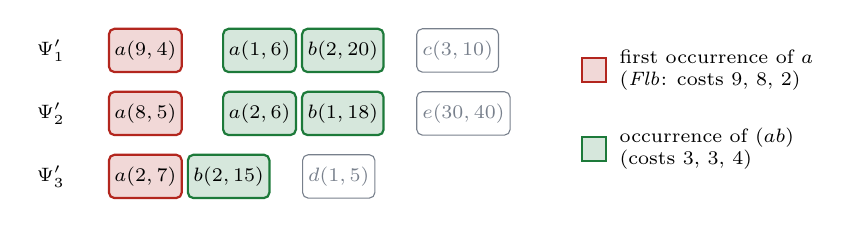
\begin{tikzpicture}[
  qi/.style={draw, rounded corners=2pt, minimum height=5.5mm, inner sep=2pt, font=\scriptsize},
  first/.style={qi, fill=badc!18, draw=badc, thick},
  occ/.style={qi, fill=okc!18, draw=okc, thick},
  plain/.style={qi, draw=grayc, text=grayc},
  lab/.style={font=\scriptsize, anchor=east}]
\node[lab] at (0,0) {$\Psi'_1$};
\node[first] (a11) at (0.9,0) {$a(9,4)$};
\node[occ] (a12) at (2.35,0) {$a(1,6)$}; \node[occ, right=0.5mm of a12] (b12) {$b(2,20)$};
\node[plain, right=4mm of b12] {$c(3,10)$};
\node[lab] at (0,-0.8) {$\Psi'_2$};
\node[first] at (0.9,-0.8) {$a(8,5)$};
\node[occ] (a22) at (2.35,-0.8) {$a(2,6)$}; \node[occ, right=0.5mm of a22] (b22) {$b(1,18)$};
\node[plain, right=4mm of b22] {$e(30,40)$};
\node[lab] at (0,-1.6) {$\Psi'_3$};
\node[first] (a31) at (0.9,-1.6) {$a(2,7)$}; \node[occ, right=0.5mm of a31] (b31) {$b(2,15)$};
\node[plain, right=4mm of b31] {$d(1,5)$};
\node[draw=badc, thick, fill=badc!18, minimum width=3mm, minimum height=3mm] at (6.6,-0.25) {};
\node[font=\scriptsize, anchor=west, align=left] at (6.8,-0.25) {first occurrence of $a$\\(\flb: costs 9, 8, 2)};
\node[draw=okc, thick, fill=okc!18, minimum width=3mm, minimum height=3mm] at (6.6,-1.25) {};
\node[font=\scriptsize, anchor=west, align=left] at (6.8,-1.25) {occurrence of $(ab)$\\(costs 3, 3, 4)};
\end{tikzpicture}
\caption{Why \flb{} is not monotone. With $m = 2$, $\flb(\seq{a}) = 5 > \flb(\seq{(ab)}) = 3$:
the occurrences of $(ab)$ do not contain the (expensive) first occurrence of $a$. In
$\Psi'_3$ the first occurrence of $a$ is also part of $(ab)$.}
\label{fig:flb}
\end{figure}

%=====================================================================
\section{A Lower Bound Based on the Cheapest Occurrence}\label{sec:mlb}
%=====================================================================

\begin{definition}[MLB]
For $\Psi' \in \rho(\alpha)$, let $\lbmin(\alpha,\Psi') = \min_{\alpha' \in O(\alpha,\Psi')}
c(\alpha')$ be the cost of the cheapest occurrence of $\alpha$ in $\Psi'$. For a sequence with
$\supp(\alpha) \ge m$, $\mlb(\alpha)$ is the average of the $m$ smallest values
$\lbmin(\alpha,\Psi')$, $\Psi' \in \rho(\alpha)$.
\end{definition}

\begin{example}
In Table~\ref{tab:toy}, $\lbmin(\seq{a},\Psi'_1) = 1$, $\lbmin(\seq{a},\Psi'_2) = 2$ and
$\lbmin(\seq{a},\Psi'_3) = 2$, so $\mlb(\seq{a}) = 1.5$, while $\flb(\seq{a}) = 5$.
For the item $e$, $\mlb(\seq{e}) = (25 + 30)/2 = 27.5$.
\end{example}

\begin{lemma}\label{lem:occ}
Let $\beta$ be a super-sequence of $\alpha$ and $\Psi' \in \rho(\beta)$. Then
$c(\beta,\Psi') \ge \lbmin(\beta,\Psi') \ge \lbmin(\alpha,\Psi')$.
\end{lemma}
\begin{proof}
The first inequality holds because a maximum is at least a minimum over the same non-empty set.
Let $\beta'$ be an occurrence of $\beta$ in $\Psi'$. Since $\alpha$ is contained in $\beta$,
the q-items of $\beta'$ that match the items of $\alpha$ form an occurrence $\alpha'$ of
$\alpha$ in $\Psi'$, and $c(\beta') \ge c(\alpha')$ because costs are positive. Hence
$c(\beta') \ge \lbmin(\alpha,\Psi')$ for every occurrence $\beta'$, and the result follows by
taking the minimum over $\beta'$. \qed
\end{proof}

\begin{theorem}[Properties of MLB]\label{thm:mlb}
Let $\alpha$ be a sequence with $\supp(\alpha) \ge m$.
(a) $\mlb(\alpha) \le \ac(\alpha)$.
(b) For every super-sequence $\beta$ of $\alpha$ with $\supp(\beta) \ge m$,
$\mlb(\beta) \ge \mlb(\alpha)$, hence $\ac(\beta) \ge \mlb(\alpha)$.
\end{theorem}
\begin{proof}
(a) Let $s = \supp(\alpha) \ge m$. By Lemma~\ref{lem:occ} (with $\beta = \alpha$), each value
$c(\alpha,\Psi')$ is at least $\lbmin(\alpha,\Psi')$, so $\ac(\alpha)$ is at least the average
of the $s$ values $\lbmin(\alpha,\Psi')$, which is at least the average of the $m$ smallest
of them.
(b) Since $\beta$ contains $\alpha$, $\rho(\beta) \subseteq \rho(\alpha)$. Let
$\Psi'_{1}, \dots, \Psi'_{m}$ be the q-sequences of $\rho(\beta)$ with the $m$ smallest values
$\lbmin(\beta,\cdot)$. By Lemma~\ref{lem:occ}, $\lbmin(\beta,\Psi'_j) \ge
\lbmin(\alpha,\Psi'_j)$ for each $j$, and the $m$ distinct q-sequences $\Psi'_j$ belong to
$\rho(\alpha)$, so $\sum_j \lbmin(\alpha,\Psi'_j)$ is at least the sum of the $m$ smallest
values $\lbmin(\alpha,\cdot)$. Thus $\mlb(\beta) \ge \mlb(\alpha)$, and
$\ac(\beta) \ge \mlb(\beta) \ge \mlb(\alpha)$ by (a). \qed
\end{proof}

Theorem~\ref{thm:mlb}(b) holds for \emph{all} super-sequences, which is the same kind of
property as the anti-monotonicity of \amub{} and of the support used by the width pruning
strategies of \FL{}. It therefore yields the following strategies, whose proofs repeat those
of the corresponding strategies of \cite[Section~4.3]{truong2022} with \mlb{} in place of
\amub{}.

\begin{corollary}[Cost-aware pruning strategies]\label{cor:strategies}
\begin{enumerate}
\item \emph{Depth pruning.} If $\mlb(\alpha) > \maxc$, no super-sequence of $\alpha$ (in
  particular no node of the subtree of $\alpha$) is an FLCHU sequence.
\item \emph{Item removal.} If $\supp(\seq{y}) < m$, $\amub(\seq{y}) < \minu$ or
  $\mlb(\seq{y}) > \maxc$, no FLCHU sequence contains $y$, and $y$ can be removed from $D'$.
  Removing items lowers the utilities $u(\Psi')$ and thus \amub{} for the remaining items,
  while supports and \mlb{} values are unchanged; the removal can therefore be repeated until
  no item is removed.
\item \emph{Co-occurrence maps.} If $\mlb(\seq{(xy)}) > \maxc$ (resp.
  $\mlb(\seq{x \to y}) > \maxc$), no i-extension (resp. s-extension) with $y$ of a sequence
  whose last item is $x$ leads to an FLCHU sequence, so $y$ can be excluded from
  $\mathit{iCMAP}(x)$ (resp. $\mathit{sCMAP}(x)$).
\item \emph{Candidate sets.} If $\mlb(\alpha \diamond y) > \maxc$, $y$ can be excluded from
  the candidate set $I(\alpha)$ or $S(\alpha)$, and therefore from the candidate sets of all
  descendants of $\alpha$ (tightening strategy of \cite{truong2022}).
\end{enumerate}
\end{corollary}

\begin{example}
With $\mins = 2$, $\minu = 20$ and $\maxc = 4$, item $e$ passes the width tests of \FL{}
($\supp = 2$ and $\amub(\seq{e}) = 63$) but $\mlb(\seq{e}) = 27.5 > \maxc$, so \FX{} removes $e$.
The utilities of $\Psi'_2$ and $\Psi'_3$ become 29 and 27, and $\amub(\seq{a})$ decreases from
63 to 34.5. In the same way, $\mlb(\seq{b \to c}) = (5 + 5)/2 = 5$ and
$\mlb(\seq{b \to d}) = (3 + 7)/2 = 5$ exceed \maxc, so $c, d \notin \mathit{sCMAP}(b)$.
\end{example}

\begin{table}[t]
\centering
\caption{Pruning tests of \FL{} and \FX{} ($\checkmark$: used; $\times$: not used).}
\label{tab:tests}
\setlength{\tabcolsep}{4pt}
\resizebox{\textwidth}{!}{\begin{tabular}{@{}llccc@{}}
\toprule
Use & Test & Valid for & \FL{} & \FX{} \\
\midrule
Depth pruning & $\fub < \minu$ & forward ext. & $\checkmark$ & $\checkmark$ \\
Depth pruning & $\flb > \maxc$ & \textcolor{badc}{no (Prop.~\ref{prop:cex})} & $\checkmark$ & $\times$ \\
Depth pruning & $\mlb > \maxc$ & all super-seq. & $\times$ & $\checkmark$ \\
Width, items, CMAPs & $\supp < \mins$, $\amub < \minu$ & all super-seq. & $\checkmark$ & $\checkmark$ \\
Width, items, CMAPs & $\mlb > \maxc$ & all super-seq. & $\times$ & $\checkmark$ \\
Item removal to a fixpoint & -- & -- & $\times$ & $\checkmark$ \\
\bottomrule
\end{tabular}}
\end{table}

%=====================================================================
\section{The FLCHUS-X Algorithm}\label{sec:algo}
%=====================================================================

\subsection{The CUL structure with cheapest costs}

\FX{} uses the CUL (cost-utility list) structure of \FL{} \cite[Section~5.1]{truong2022}. For a
sequence $\alpha$ and $\Psi' \in \rho(\alpha)$, the CUL stores one tuple per ending position
$e$ of $\alpha$ in $\Psi'$, containing the maximum cost $c_e$ and the maximum utility $u_e$ of
the occurrences of $\alpha$ that end at $e$, and the utility $\mathit{ru}_e$ of the rest of
$\Psi'$. \FX{} adds one field: the cost $\mathit{cm}_e$ of the cheapest occurrence ending at
$e$. Then $u(\alpha,\Psi') = \max_e u_e$, $c(\alpha,\Psi') = \max_e c_e$,
$\lbmin(\alpha,\Psi') = \min_e \mathit{cm}_e$, and the bound of \fub{} is
$\max_e (u_e + \mathit{ru}_e)$.

\begin{lemma}[CUL of extensions]\label{lem:cul}
Let $t_y$ be the tuple of item $y$ at position $e$ in $\Psi'$, with cost $c(y)$. For the
i-extension $\beta = \alpha \diamond_i y$, the tuple of $\beta$ at $e$ exists if $\alpha$ has a
tuple $t_\alpha$ at $e$, and $\mathit{cm}_e(\beta) = \mathit{cm}_e(\alpha) + c(y)$. For the
s-extension $\beta = \alpha \diamond_s y$, it exists if $\alpha$ has a tuple at a position
$e' < e$, and $\mathit{cm}_e(\beta) = \min_{e' < e} \mathit{cm}_{e'}(\alpha) + c(y)$.
\end{lemma}
\begin{proof}
Every occurrence of $\beta$ ending at $e$ consists of an occurrence of $\alpha$ ending at $e$
(i-extension) or at some $e' < e$ (s-extension), plus the q-item of $y$ at $e$; conversely
every such combination is an occurrence of $\beta$ (for an i-extension, $y$ is greater than the
items of the last itemset of $\alpha$). Since the cost of the combination is the sum of the two
costs, the minimum over the occurrences ending at $e$ is the minimum of the costs of $\alpha$
plus $c(y)$. \qed
\end{proof}

The maximum cost and utility of extensions are computed in the same way with maxima
\cite[Section~5.1.3]{truong2022}. Figure~\ref{fig:cul} shows the CULs of $a$, $b$ and $(ab)$ of
the toy QSDB after the removal of $e$.

\begin{figure}[t]
\centering
\scriptsize
\resizebox{0.95\textwidth}{!}{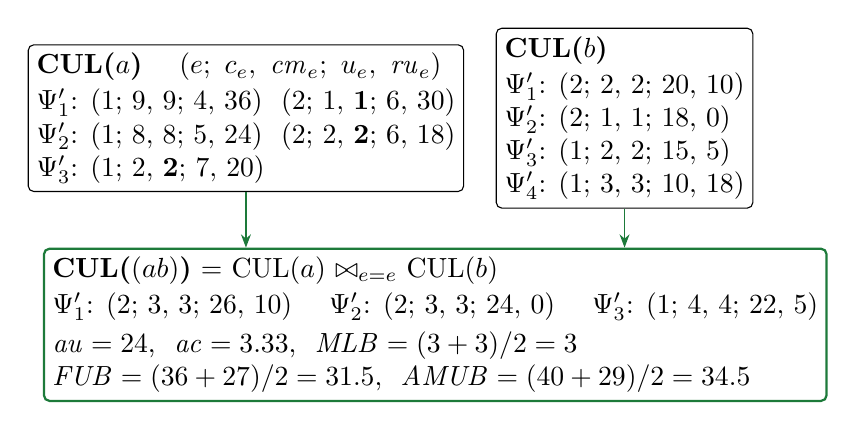
\begin{tikzpicture}[node distance=4mm]
\node[draw, rounded corners=2pt, align=left, inner sep=3pt] (A) {
\textbf{CUL($a$)} \quad $(e;\ c_e,\ \mathit{cm}_e;\ u_e,\ \mathit{ru}_e)$\\[1pt]
$\Psi'_1$: $(1;\,9,\,9;\,4,\,36)$ \ $(2;\,1,\,\mathbf{1};\,6,\,30)$\\
$\Psi'_2$: $(1;\,8,\,8;\,5,\,24)$ \ $(2;\,2,\,\mathbf{2};\,6,\,18)$\\
$\Psi'_3$: $(1;\,2,\,\mathbf{2};\,7,\,20)$};
\node[draw, rounded corners=2pt, align=left, inner sep=3pt, right=of A] (B) {
\textbf{CUL($b$)}\\[1pt]
$\Psi'_1$: $(2;\,2,\,2;\,20,\,10)$\\
$\Psi'_2$: $(2;\,1,\,1;\,18,\,0)$\\
$\Psi'_3$: $(1;\,2,\,2;\,15,\,5)$\\
$\Psi'_4$: $(1;\,3,\,3;\,10,\,18)$};
\node[draw=okc, thick, rounded corners=2pt, align=left, inner sep=3pt, below=6mm of $(A.south)!0.5!(B.south)$] (AB) {
\textbf{CUL($(ab)$)} = CUL($a$) $\bowtie_{e=e}$ CUL($b$)\\[1pt]
$\Psi'_1$: $(2;\,3,\,3;\,26,\,10)$ \quad $\Psi'_2$: $(2;\,3,\,3;\,24,\,0)$ \quad $\Psi'_3$: $(1;\,4,\,4;\,22,\,5)$\\[2pt]
$\au = 24$, \ $\ac = 3.33$, \ $\mlb = (3+3)/2 = 3$\\
$\fub = (36+27)/2 = 31.5$, \ $\amub = (40+29)/2 = 34.5$};
\draw[-{Stealth}, okc] (A.south) -- (AB.north -| A.south);
\draw[-{Stealth}, okc] (B.south) -- (AB.north -| B.south);
\end{tikzpicture}}
\caption{CULs of $a$, $b$ and of the i-extension $(ab)$ on the toy QSDB after removing $e$.
Bold values give $\lbmin(\seq{a},\cdot) = 1, 2, 2$, hence $\mlb(\seq{a}) = 1.5$, whereas the
first occurrences of $a$ give $\flb(\seq{a}) = 5$.}
\label{fig:cul}
\end{figure}

\subsection{The algorithm}

Algorithm~\ref{alg:fx} shows \FX{}. It first computes the CULs of the items and removes items
with Corollary~\ref{cor:strategies}(2) until no item is removed (lines 1--5). It then builds the
co-occurrence maps with the support, \amub{} and \mlb{} tests (line 6) and explores the prefix
tree depth-first (procedure \textsc{Search}). For a node $\alpha$, it applies depth pruning with
\fub{} and \mlb{} (line 9), outputs $\alpha$ if it is an FLCHU sequence (line 10), and builds
the candidate sets of i- and s-extensions with the width tests (lines 11--16). The search
space, the utility bounds and the tightening of candidate sets are those of \FL{}; the
differences are the use of \mlb{} instead of \flb{}, the cost tests in lines 3, 6, 13 and 15,
and the repetition of item removal.

\begin{algorithm}[t]
\caption{\FX}\label{alg:fx}
\small
\begin{algorithmic}[1]
\Require QSDB $D'$, thresholds $\mins$, $\minu$, $\maxc$
\Ensure the set of FLCHU sequences
\Repeat
  \State compute $u(\Psi')$ for all $\Psi' \in D'$ and $\mathrm{CUL}(\seq{y})$ for all items $y$
  \State $R \gets \{y \mid \supp(\seq{y}) < \mins \lor \amub(\seq{y}) < \minu \lor \mlb(\seq{y}) > \maxc\}$
  \State remove the items of $R$ from $D'$
\Until{$R = \emptyset$}
\State compute $\mathit{iCMAP}$ and $\mathit{sCMAP}$ with the tests on $\supp$, \amub{} and \mlb{}
\State $S \gets$ items of $D'$; \textbf{for each} $x \in S$ \textbf{do} \Call{Search}{$\seq{x}, S, S$}
\Procedure{Search}{$\alpha, I, S$}
  \If{$\fub(\alpha) < \minu \lor \mlb(\alpha) > \maxc$} \Return \EndIf
  \If{$\au(\alpha) \ge \minu \land \ac(\alpha) \le \maxc$} output $\alpha$ \EndIf
  \State $x \gets$ last item of $\alpha$; $I(\alpha) \gets \emptyset$; $S(\alpha) \gets \emptyset$
  \ForAll{$y \in I$, $y \succ x$, $y \in \mathit{iCMAP}(x)$}
    \If{$\supp(\alpha\diamond_i y) \ge \mins \land \amub(\alpha\diamond_i y) \ge \minu \land \mlb(\alpha\diamond_i y) \le \maxc$} $I(\alpha) \gets I(\alpha) \cup \{y\}$ \EndIf
  \EndFor
  \ForAll{$y \in S$, $y \in \mathit{sCMAP}(x)$}
    \If{$\supp(\alpha\diamond_s y) \ge \mins \land \amub(\alpha\diamond_s y) \ge \minu \land \mlb(\alpha\diamond_s y) \le \maxc$} $S(\alpha) \gets S(\alpha) \cup \{y\}$ \EndIf
  \EndFor
  \ForAll{$y \in I(\alpha)$} \Call{Search}{$\alpha \diamond_i y, I(\alpha), S(\alpha)$} \EndFor
  \ForAll{$y \in S(\alpha)$} \Call{Search}{$\alpha \diamond_s y, S(\alpha), S(\alpha)$} \EndFor
\EndProcedure
\end{algorithmic}
\end{algorithm}

\begin{theorem}
\FX{} outputs exactly the set of FLCHU sequences.
\end{theorem}
\begin{proof}
Every output sequence satisfies the three conditions (line 10), with values computed exactly
from the CULs (Lemma~\ref{lem:cul} and \cite[Section~5.1]{truong2022}). Completeness: the
search space is the prefix tree of all sequences over the items of $D'$; a subtree is pruned
or an item is skipped only by a test that, by \cite[Theorems~1 and 3]{truong2022} for the
support, \amub{} and \fub{}, and by Theorem~\ref{thm:mlb} and Corollary~\ref{cor:strategies}
for \mlb{}, guarantees that the skipped sequences are not FLCHU sequences. \qed
\end{proof}

\paragraph{Implementation details.} The bounds need the sum of the $m$ largest (or smallest)
values over the q-sequences of a CUL. \FX{} obtains it with a linear-time selection instead of
sorting, and stops the construction of an extension's CUL as soon as fewer than $m$ q-sequences
can still contain it. Neither change affects the output.

\subsection{Running example}

Figure~\ref{fig:tree} compares the nodes visited by \FL{} and by \FX{} on the toy QSDB
($\mins = 2$, $\minu = 20$, $\maxc = 4$). With \flb-based depth pruning, the subtree of
$\seq{a}$ is pruned, so $\seq{(ab)}$ is not reached, and the nodes $\seq{e}$, $\seq{b \to c}$,
$\seq{b \to d}$ and $\seq{b \to e}$ are visited before being pruned; 8 nodes are visited. \FX{}
removes $e$ before the search and excludes $c$ and $d$ from $\mathit{sCMAP}(b)$, since their
\mlb{} values exceed \maxc; it visits 5 nodes and outputs $\seq{(ab)}$. The values in the figure
were computed by the implementations described in Section~\ref{sec:exp}.

\begin{figure}[t]
\centering
\scriptsize
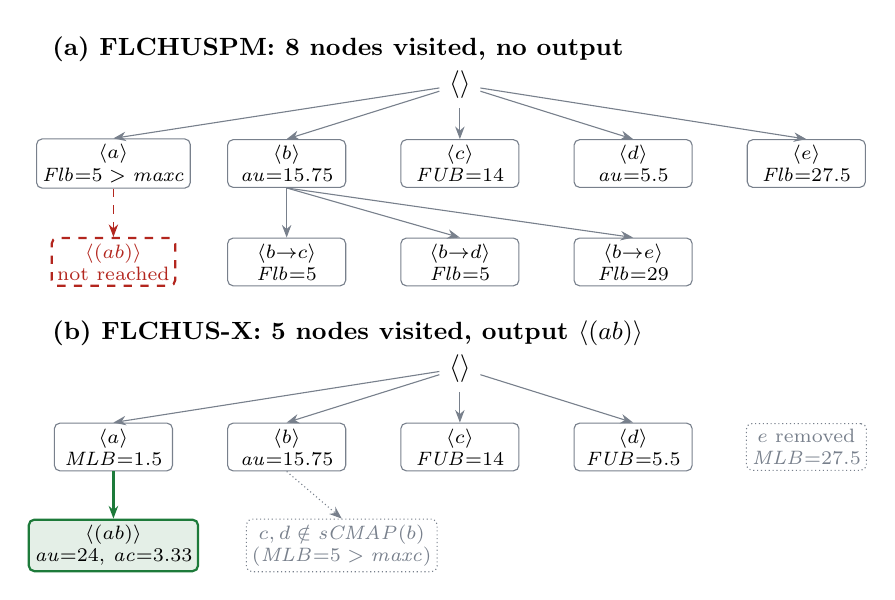
\begin{tikzpicture}[
  nd/.style={draw, rounded corners=2pt, inner sep=2pt, align=center, minimum width=15mm, font=\scriptsize},
  pr/.style={nd, draw=grayc},
  bad/.style={nd, draw=badc, dashed, text=badc, thick},
  sol/.style={nd, draw=okc, thick, fill=okc!12},
  gone/.style={nd, draw=grayc, densely dotted, text=grayc},
  e/.style={-{Stealth[length=1.6mm]}, grayc}]
% (a) FLCHUSPM
\node[font=\small\bfseries, anchor=west] at (-0.9,0.45) {(a) \FL{}: 8 nodes visited, no output};
\node (r1) at (4.4,0) {$\seq{}$};
\node[pr] (a1) at (0,-1) {$\seq{a}$\\ $\flb{=}5 > \maxc$};
\node[pr] (b1) at (2.2,-1) {$\seq{b}$\\ $\au{=}15.75$};
\node[pr] (c1) at (4.4,-1) {$\seq{c}$\\ $\fub{=}14$};
\node[pr] (d1) at (6.6,-1) {$\seq{d}$\\ $\au{=}5.5$};
\node[pr] (e1) at (8.8,-1) {$\seq{e}$\\ $\flb{=}27.5$};
\node[bad] (ab1) at (0,-2.25) {$\seq{(ab)}$\\ not reached};
\node[pr] (bc1) at (2.2,-2.25) {$\seq{b{\to}c}$\\ $\flb{=}5$};
\node[pr] (bd1) at (4.4,-2.25) {$\seq{b{\to}d}$\\ $\flb{=}5$};
\node[pr] (be1) at (6.6,-2.25) {$\seq{b{\to}e}$\\ $\flb{=}29$};
\foreach \x in {a1,b1,c1,d1,e1} \draw[e] (r1) -- (\x.north);
\draw[e, badc, dashed] (a1) -- (ab1);
\foreach \x in {bc1,bd1,be1} \draw[e] (b1.south) -- (\x.north);
% (b) FLCHUS-X
\begin{scope}[yshift=-3.6cm]
\node[font=\small\bfseries, anchor=west] at (-0.9,0.45) {(b) \FX{}: 5 nodes visited, output $\seq{(ab)}$};
\node (r2) at (4.4,0) {$\seq{}$};
\node[pr] (a2) at (0,-1) {$\seq{a}$\\ $\mlb{=}1.5$};
\node[pr] (b2) at (2.2,-1) {$\seq{b}$\\ $\au{=}15.75$};
\node[pr] (c2) at (4.4,-1) {$\seq{c}$\\ $\fub{=}14$};
\node[pr] (d2) at (6.6,-1) {$\seq{d}$\\ $\fub{=}5.5$};
\node[gone] (e2) at (8.8,-1) {$e$ removed\\ $\mlb{=}27.5$};
\node[sol] (ab2) at (0,-2.25) {$\seq{(ab)}$\\ $\au{=}24$, $\ac{=}3.33$};
\node[gone] (bc2) at (2.9,-2.25) {$c, d \notin \mathit{sCMAP}(b)$\\ ($\mlb{=}5 > \maxc$)};
\foreach \x in {a2,b2,c2,d2} \draw[e] (r2) -- (\x.north);
\draw[e, okc, thick] (a2) -- (ab2);
\draw[e, densely dotted] (b2.south) -- (bc2.north);
\end{scope}
\end{tikzpicture}
\caption{Nodes visited on the toy QSDB with $\mins = 2$, $\minu = 20$, $\maxc = 4$. Gray: node
visited and not output (the value shown is the reason); green: FLCHU sequence; red dashed:
FLCHU sequence not reached; dotted: pruned before the search.}
\label{fig:tree}
\end{figure}

\subsection{Complexity}

As in \FL{}, the CUL of an extension is built by a merge of two CULs in time linear in their
number of tuples, and the measures of a node are computed in time linear in the size of its
CUL; the selection of the $m$ extreme values takes linear expected time instead of
$O(n \log n)$ for a sort over $n$ q-sequences. \FX{} adds one value per tuple
($\mathit{cm}_e$) to the CULs of \FL{}. Item removal is repeated at most $|A|$ times, each time with a scan of
$D'$; in the experiments it converged in \todo{number of rounds} rounds.

%=====================================================================
\section{Experimental Evaluation}\label{sec:exp}
%=====================================================================

\FX{} and \FL{} were implemented in C in the same framework, sharing the input parser and the
CUL construction; \FL{} follows Definitions 4--6, Theorems 1--3, Section 5.1 and Figs.~3--4 of
\cite{truong2022}. As no implementation of \FL{} is publicly available, it was implemented from
\cite{truong2022} and validated on the running example of that paper: the implementation returns
the published result, the CULs of all items of \cite[Fig.~1]{truong2022}, the published
co-occurrence maps, and the 14 nodes of \cite[Fig.~5]{truong2022}; the bound values agree
except two \flb{} values of pruned nodes, for which the figure reports values equal to the \ac{}
values of other nodes. Two algorithms are compared: \FL{}, and \FL{} without the \flb{}
test (denoted \FL$^{-}$), which is sound and is the correct baseline. \todo{hardware and
software environment}

\subsection{Correctness}

A brute-force implementation of the problem definition (Definitions 1--4 of \cite{truong2022})
enumerates every sequence with support at least \mins{} and computes its utility and cost from
all its occurrences. It was compared with the algorithms on random QSDBs with 2 to 7
q-sequences of 1 to 5 itemsets over 2 to 5 items, random costs in $[1,20]$, utilities in
$[1,50]$ and random thresholds. Table~\ref{tab:oracle} reports the results.

\begin{table}[t]
\centering
\caption{Comparison with the brute-force implementation (number of databases where the output
differs; missing / extra patterns / patterns with different values).}
\label{tab:oracle}
\begin{tabular}{@{}lrrrrrr@{}}
\toprule
Algorithm & Databases & FLCHU seq. & Differing & Missing & Extra & Values \\
\midrule
\FL{} & 500 & 21{,}807 & 2 & 2 & 0 & 0 \\
\FL$^{-}$ & 500 & 21{,}807 & 0 & 0 & 0 & 0 \\
\FX{} & 500 & 21{,}807 & 0 & 0 & 0 & 0 \\
\FX{} (second seed) & 1{,}000 & 53{,}439 & 0 & 0 & 0 & 0 \\
\bottomrule
\end{tabular}
\end{table}

The two databases where \FL{} differs both contain an i-extension whose prefix is pruned by
\flb{} as in Proposition~\ref{prop:cex}; each of the three strategies of \FX{} was also
disabled in turn, and the output was identical to the brute force in all 500 databases.

\subsection{Datasets}

The datasets of \cite{truong2022} include BMS, Snake and three synthetic datasets generated
with the IBM Quest generator; the synthetic files are not publicly available. BMS and Snake and
four other real sequence datasets commonly used in sequential pattern mining were used, all
obtained from the SPMF library website \cite{fournier2016spmf} (Table~\ref{tab:data}; BMS and
Snake match the characteristics reported in \cite{truong2022}). As in \cite{truong2022}, costs
and utilities of q-items were generated in $[1, 70]$ and $[10, 100]$ with a log-normal
distribution; since its parameters are not given in \cite{truong2022}, each q-item received $\exp(Y)$ rounded, where $Y$ is normal with the interval of logarithms as $\pm 3$
standard deviations, truncated to the interval.

\begin{table}[t]
\centering
\caption{Characteristics of the datasets.}
\label{tab:data}
\begin{tabular}{@{}lrrrr@{}}
\toprule
Dataset & \#sequences & \#items & avg.\ length & (min; max) length \\
\midrule
BMS & 59{,}601 & 497 & 2.5 & (1; 267) \\
Snake & 163 & 20 & 60.6 & (57; 61) \\
SIGN & 730 & 267 & 52.0 & (18; 94) \\
FIFA & 20{,}450 & 2{,}990 & 36.2 & (9; 100) \\
LEVIATHAN & 5{,}834 & 9{,}025 & 33.8 & (9; 100) \\
BIBLE & 36{,}369 & 13{,}905 & 21.6 & (9; 100) \\
\bottomrule
\end{tabular}
\end{table}

\subsection{Runtime, memory and search space}

\todo{Runtime and peak memory of \FL{}, \FL$^{-}$ and \FX{} when varying \mins{}, \minu{}
and \maxc{} on each dataset (median of three runs, single thread, time limit), number of
visited nodes and of constructed extensions.
The benchmark has not been run yet; no performance result is claimed in this draft.}

\subsection{Ablation study}

\todo{Runtime of \FX{} with each of the three strategies disabled (cost-aware width pruning,
repeated item removal, linear-time selection and early abandon).}

%=====================================================================
\section{Conclusion}\label{sec:concl}
%=====================================================================

This paper studied lower bounds on the average cost for the FLCHUSM problem of Truong et al.\
\cite{truong2022}. The lower bound \mlb{}, based on the cheapest occurrence of a sequence, is
monotone for all super-sequences, which allows using the cost not only for depth pruning but
also for removing items, filtering the co-occurrence maps and tightening the candidate sets. The
analysis also showed that a bound based on the first occurrence is not monotone for
i-extensions. The resulting algorithm, \FX{}, returned the same output as a brute-force
implementation of the problem definition on all tested databases.
\todo{summary of the performance results}. Future work includes tighter bounds that combine
cost and utility, and the extension of \mlb{} to other cost-aware pattern mining tasks.

\begin{thebibliography}{10}

\bibitem{agrawal1995}
Agrawal, R., Srikant, R.: Mining sequential patterns. In: Proceedings of the Eleventh
International Conference on Data Engineering, pp. 3--14 (1995).
\doi{10.1109/ICDE.1995.380415}

\bibitem{fournier2014cmap}
Fournier-Viger, P., Gomariz, A., Campos, M., Thomas, R.: Fast vertical mining of sequential
patterns using co-occurrence information. In: Advances in Knowledge Discovery and Data Mining
(PAKDD 2014), LNCS, pp. 40--52. Springer (2014). \doi{10.1007/978-3-319-06608-0_4}

\bibitem{fournier2016spmf}
Fournier-Viger, P., Lin, J.C.W., Gomariz, A., Gueniche, T., Soltani, A., Deng, Z.: The SPMF
open-source data mining library version 2. In: Machine Learning and Knowledge Discovery in
Databases (ECML PKDD 2016), LNCS, pp. 36--40. Springer (2016).
\doi{10.1007/978-3-319-46131-1_8}

\bibitem{fournier2020cost}
Fournier-Viger, P., Li, J., Lin, J.C.W., Truong Chi, T., Uday Kiran, R.: Mining cost-effective
patterns in event logs. Knowledge-Based Systems \textbf{191}, 105241 (2020).
\doi{10.1016/j.knosys.2019.105241}

\bibitem{gan2021survey}
Gan, W., Lin, J.C.W., Fournier-Viger, P., Chao, H.C., Tseng, V.S., Yu, P.S.: A survey of
utility-oriented pattern mining. IEEE Transactions on Knowledge and Data Engineering
\textbf{33}(4), 1306--1327 (2021). \doi{10.1109/TKDE.2019.2942594}

\bibitem{nawaz2022lcim}
Nawaz, M.S., Fournier-Viger, P., Alhusaini, N., He, Y., Wu, Y., Bhattacharya, D.: LCIM:
Mining low cost high utility itemsets. In: Multi-disciplinary Trends in Artificial
Intelligence (MIWAI 2022), LNCS, pp. 73--85. Springer (2022).
\doi{10.1007/978-3-031-20992-5_7}

\bibitem{pei2004}
Pei, J., Han, J., Mortazavi-Asl, B., Wang, J., Pinto, H., Chen, Q., Dayal, U., Hsu, M.C.:
Mining sequential patterns by pattern-growth: the PrefixSpan approach. IEEE Transactions on
Knowledge and Data Engineering \textbf{16}(11), 1424--1440 (2004).
\doi{10.1109/TKDE.2004.77}

\bibitem{truong2022}
Truong, T., Duong, H., Le, B., Fournier-Viger, P., Yun, U.: Mining interesting sequences with
low average cost and high average utility. Applied Intelligence \textbf{52}(7), 7136--7157
(2022). \doi{10.1007/s10489-021-02505-0}

\bibitem{yin2012uspan}
Yin, J., Zheng, Z., Cao, L.: USpan: an efficient algorithm for mining high utility sequential
patterns. In: Proceedings of the 18th ACM SIGKDD International Conference on Knowledge
Discovery and Data Mining, pp. 660--668 (2012). \doi{10.1145/2339530.2339636}

\bibitem{zaki2001}
Zaki, M.J.: SPADE: An efficient algorithm for mining frequent sequences. Machine Learning
\textbf{42}(1--2), 31--60 (2001). \doi{10.1023/A:1007652502315}

\end{thebibliography}
\end{document}
